A recommender system is a type of data-driven, intelligent application addressing the information overload phenomenon on the internet. The application selects top items that are the most likely to be desired by target users under a specific metric, and it assists users' behavior on online services. Most importantly, the foundation of the recommendation engine relies on simple vector and matrix computation against sparse user-item data, where we can take full advantage of numerical computing methods. That is, many classic but still performant recommendation algorithms run on a $|\mathcal{U}|$-by-$|\mathcal{I}|$ user-item matrix $R \in \mathbb{R}^{|\mathcal{U}| \times |\mathcal{I}|}$, where $\mathcal{U}$ and $\mathcal{I}$ are respectively a set of users and items. Notice that $R$ normally shows high sparsity with limited user-item events on massive $|\mathcal{U}|$ and $|\mathcal{I}|$. \fig{recommender} illustrates how user-item data is transformed and processed for making recommendations.

\begin{figure}[htbp]
    \centering
    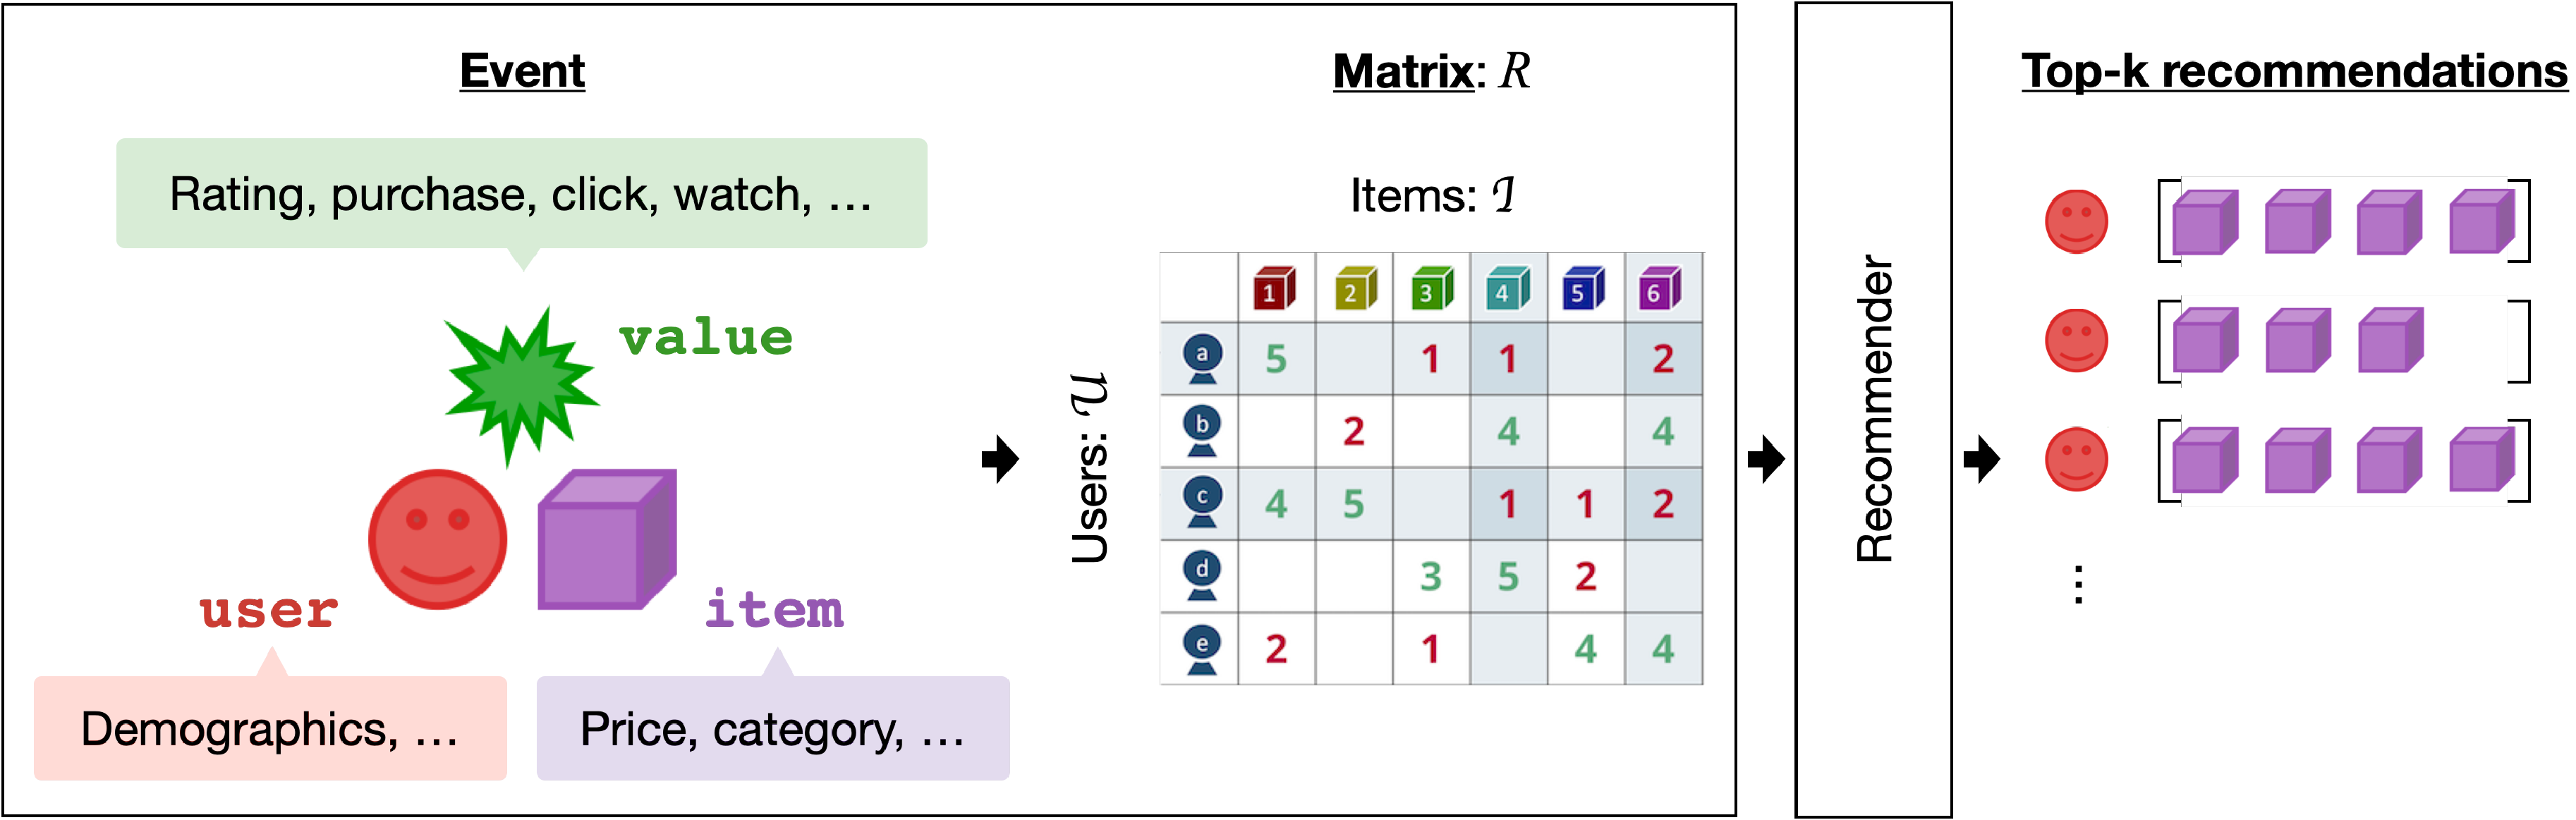
\includegraphics[width=1.0\linewidth]{images/recommender.pdf}
    \caption{Overview of how a recommender works. Event data between users and items are converted into a matrix $R$, which is eventually fed into a recommendation algorithm to generate a ranked list of items per user.}
    \label{fig:recommender}
\end{figure}

Therefore, the Julia programming language that focuses on high-performance scientific computing by utilizing the just-in-time compiler \cite{bezanson2017julia} can be a great choice for developers to efficiently and effectively pre-process user-item data, build a recommendation model, evaluate a ranked list of recommended contents, and post-process the recommendation if needed. Conventionally, MATLAB\footnote{\url{http://www.mathworks.com/}} has been widely used for numerical computing, but it is in some sense inefficient proprietary software. Alternatively, open-sourced Julia's efficient implementation is getting the attention of research communities these days. We can readily use various scientific algorithms in Julia by integrating third-party packages, and its syntax dedicated to vector and matrix computations strongly accelerates algorithm development both in industry and academia. However, when it comes to building recommender systems, there are currently no effective Julia packages that enable us to implement recommendation functionality in an extensible way to the best of the author's knowledge.

For the reasons mentioned above, \texttt{Recommendation.jl}\footnote{\url{https://github.com/takuti/Recommendation.jl/}} has been developed in the unique Julia ecosystem. It should be noted that there are quite a few non-Julia open-source solutions available in the community. To give an example, \texttt{LensKit} \cite{ekstrand2020lenskit} takes full advantage of the NumPy/SciPy-based Python scientific computing ecosystem, which naturally makes rapid development and wider use cases possible. On the other hand, \texttt{MyMediaLite} \cite{gantner2011mymedialite} written in C\# is one of the most classic examples that rely purely on the language's built-in arithmetic operators with file IOs; although the tool maximizes the simplicity and transparency of basic recommendation techniques, it is not straightforward for developers to customize the implementation and apply the advanced techniques for optimizing further. Meanwhile, in Java, \texttt{LibRec} \cite{guo2015librec} implements custom interfaces (e.g., dense/sparse matrices) from scratch, and it allows the tool to ensure high extensibility and support various types of state-of-the-art recommenders. 

Regardless of the choice of package, practitioners will realize the recommender implementation can be broken down into similar sub-components: data, recommender, and metrics. \fig{components} illustrates the point, and the rest of the paper is accordingly organized as follows. First, \sect{data} shows how the package eases data manipulation by providing a unified abstraction layer, namely \texttt{DataAccessor}. Next, \sect{algorithm} reviews a variety of recommendation methods the package supports, including collaborative filtering, matrix factorization, and factorization machines. Moreover, in \sect{evaluation}, we dive deep into some of the recommender-specific evaluation metrics and their implementation in Julia, which enable developers to optimize recommenders against not only standard accuracy metrics (e.g., recall, precision) but non-accuracy measures such as novelty, diversity, and serendipity. Finally, \sect{experiment} provides comprehensive benchmark results for supported recommender-metric pairs to undergo trade-off discussion. 

\begin{figure}[htbp]
    \centering
    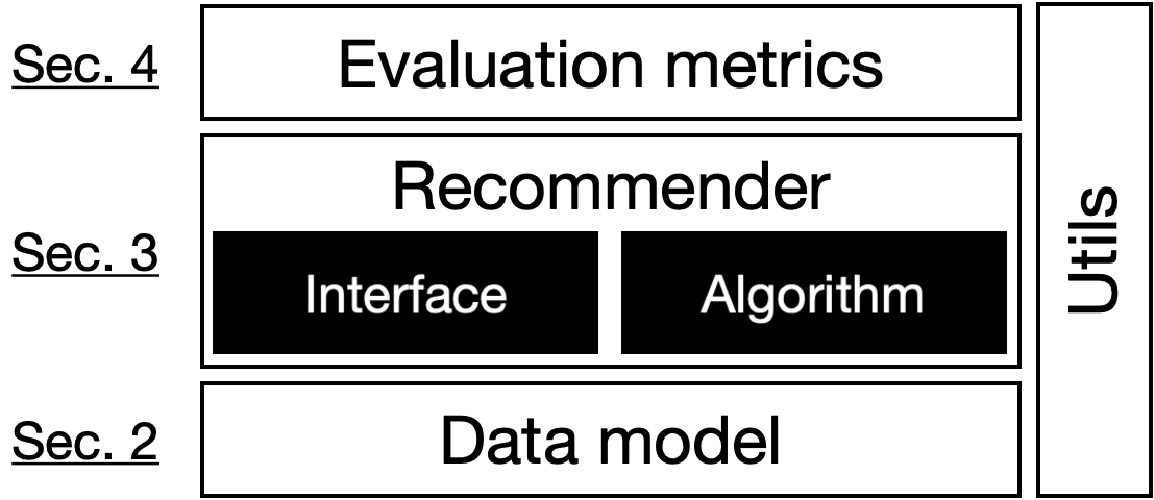
\includegraphics[width=0.5\linewidth]{images/components.pdf}
    \caption{Core components of practical recommender systems. We review each of them throughout the paper.}
    \label{fig:components}
\end{figure}

Ultimately, the contribution of this paper includes but is not limited to (1) demonstrating the Julia-based recommender package that had never existed, (2) sharing the scientific background of the field of recommender systems with the Julia community, and (3) lowering the bar to use the unique programming language in real-world applications as \texttt{Recommendation.jl} has already been used in the hands-on tutorial books \cite{balbaert2019julia,salceanu2018julia}. It should be noted that this paper assumes using \texttt{Recommendation.jl@v1.0.0}, meaning the details might differ in different versions.
